%
% File naacl2019.tex
%
%% Based on the style files for ACL 2018 and NAACL 2018, which were
%% Based on the style files for ACL-2015, with some improvements
%%  taken from the NAACL-2016 style
%% Based on the style files for ACL-2014, which were, in turn,
%% based on ACL-2013, ACL-2012, ACL-2011, ACL-2010, ACL-IJCNLP-2009,
%% EACL-2009, IJCNLP-2008...
%% Based on the style files for EACL 2006 by 
%%e.agirre@ehu.es or Sergi.Balari@uab.es
%% and that of ACL 08 by Joakim Nivre and Noah Smith

\documentclass[11pt,a4paper]{article}
\usepackage[hyperref]{naaclhlt2019}
\usepackage{times}
\usepackage{latexsym}
\usepackage{graphicx}
\usepackage{multirow}
\usepackage{url}
\usepackage{float} 
%\aclfinalcopy % Uncomment this line for the final submission
%\def\aclpaperid{***} %  Enter the acl Paper ID here

%\setlength\titlebox{5cm}
% You can expand the titlebox if you need extra space
% to show all the authors. Please do not make the titlebox
% smaller than 5cm (the original size); we will check this
% in the camera-ready version and ask you to change it back.

\newcommand\BibTeX{B{\sc ib}\TeX}

\title{Sparse Word Embedding for Multi-domain Machine Translation}

\author{Minh Quang Pham\\
  Affiliation / Address line 1 \\
  Affiliation / Address line 2 \\
  Affiliation / Address line 3 \\
  {\tt email@domain} \\\And
  Second Author \\
  Affiliation / Address line 1 \\
  Affiliation / Address line 2 \\
  Affiliation / Address line 3 \\
  {\tt email@domain} \\}

\date{}

\begin{document}
\maketitle
\begin{abstract}
In this paper, we introduce an application of an old technique \cite{P07-1033} in Multi-Domain Neural Machine Translation.  By defining general information encoding region and domain-specific encoding region in word embedding vector, we are able to  seperate domain-related information flows in forward and backward propagation during training
mitigate the catastrophic interference happens between the inference of different domains in Neural Machine Translation system, i.e to improve the performance of the system for every domain in which it was trained. 
\end{abstract}

\section{Introduction}
Despite fast improvement thanks to new architectures \cite{NIPS2017_7181} \cite{bahdanau2014neural} \cite{D13-1176} \cite{Sutskever2014Sequence}, Machine Translation still struggles with data scarcity. Domain adaptation, or it's special case Multi-domain, is the situation where in-domain data for example banking is rare while out-domain data such as news are plenty, one aims to leverage out-domain data to improve quality of Machine Translation system which is perfectible while being trained with small in-domain dataset. The problem is that we have not been able to apply Domain-adaptation to several domains at once, i.e to build one model which is best for several domains. It is obvious to realize that the bias to in-domain dataset makes model worse in translating other domains. This phenomenon can be implied by well-known problem in Machine Learning, Catastrophic Interference \cite{Michael1989Catastrophic}. In Multi-domain Machine Translation, one have to deal with polysemies whose meaning can be totally different in different domains, for example, the word "chair" means an household tool in "if you are taking a medicine which may cause low blood pressure when rising from a chair or bed " (extracted from medical corpora EMEA \cite{Tiedemann2009RANLP5}) while the word "chair" means to preside over a meeting in following sentence "The President of the ECB or , in his absence , the Vice-President , chairs the meetings of the Governing Council , the Executive Board and the General Council of the ECB. " (extracted from European Central Bank corpora \cite{Tiedemann2009RANLP5}). Using the same word embedding for polysemy obstructs the model from differentiating the meaning of a polysemy in one domain from it's other meaning in the other domain. 

\section{Related Work}
Multi-domain Machine Translation has largely interested NLP community by its promising applications in industry and its relation to fundamental problems in theory. Researchers have proposed a large range of techniques from Data centric methods to Model centric methods \cite{C18-1111}; \cite{P17-2061}. Data centric methods have goal to collect related-domain data from existing in-domain data by using different techniques such as scoring relatedness by Language Model (\cite{P10-2041}; \cite{D11-1033}; \cite{P13-2119} or by metric on the space of sentence embedding \cite{P17-2089} or generating pseudo parallel data \cite{P03-1010}; \cite{C16-1295}; \cite{D14-1023}. On the other hand, Model centric approaches focus on NMT models that are specialized for domain adaptation. The novelty can be either trainining objective \cite{Luong2015SNMT}; \cite{P16-1009}; \cite{D17-1155}; \cite{W17-3205}; \cite{D17-1156}; \cite{C18-1269} or architecture \cite{R17-1049}; \cite{gulcehre2016monolingual}; \cite{W17-4712}, \cite{Biao2017CARENMT}; \cite{N18-2080}; \cite{W18-6313}; \cite{C16-1170}; \cite{P18-2050} or the decoding algorithm \cite{gulcehre2016monolingual}; \cite{I17-2004}. Beside these works, we could also consider "out-of-domain" works such as sequence labeling tasks \cite{P07-1033}; learning multiple visual domains \cite{NIPS2017_6654}. The problem is recently investigated by several interesting works presented in EMNLP 2018 such as \cite{D18-1039}; \cite{D18-1041}. \cite{D18-1041} create in the encoder Domain-specific gate $g^r_i$and Domain-shared gate $g^s_i$ which are generated from domain-specific and domain-shared semantic representations of source sentence $E_r(x)$ and $E_s(x)$ respectively and which select information from units of hidden states $h_i$ by elementwise product $h^r_i = g^r_i \odot h_i$; $h^s_i = g^s_i \odot h_i$. $h^r_i$ and $h^s_i$ will be fed to Domain-specific and Domain-shared attentional mechanisms respectively. While introducing new features in the architecture, \cite{D18-1041} introduces also new objective which is sum of word-level weighted MT objective and objectives of Domain-classifier in source side and target side and Adversarial Domain-classifier in source side. The author have very good approach to well seperate Domain-shared information flow and Domain-specify information flow and determine their contributions to the inference that mitigates the catastrophic interference happens in the network during forward step. 

\section{The Model}
There is not any changes in the architecture of Neural Machine Translation network except the construction of word embedding. 
\begin{figure}[h]
\center
    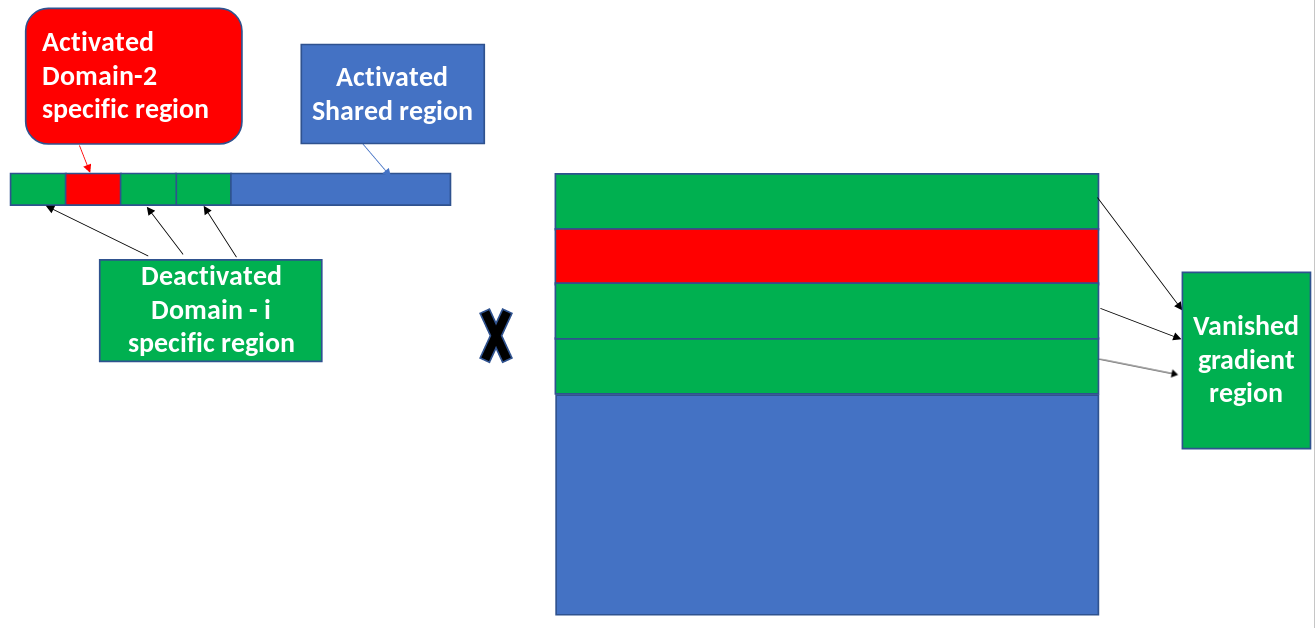
\includegraphics[width=0.8\linewidth]{Sparse1}
    \caption{Illustration of the model.} 
    \label{network}
\end{figure}
\section{Experiments}

\subsection{Corpora}
To evaluate the performance of proposed architecture, we use 4 corpora for training: European Medicines Agency; European Central Bank, News-commentary and European Parliament \cite{Tiedemann2009RANLP5} corresponding to 4 domains: medical, banking, news and administrative  respectively and one non-domain corpora Common-crawl  which was introduced in Shared Task: Machine Translation of News the Third Conference On Machine Translation 2018(WMT2018). We use Khresmoi-dev, a test set used in the Biomedical Translation Task (WMT2018), newstest2008, and test2006 as validation set for domains: medical, news administrative; except for banking domain, we use a subset of size 2000 extracted from original corpora and excluded from training set. To test the model, we use Khresmoi-test; newstest2009 and test2007 for domains: medical, news administrative; except for banking domain, we use a subset of size 2000 extracted from original corpora and excluded from training set. The information of used corpora is presented in table \ref{table:Corpora}
\begin{table}[H]
\resizebox{\columnwidth}{!}{
\begin{tabular}{ |l|l|l|l|l|l| }
\hline
Task & Corpora & Train & Dev & Test & Vocabulary \\ \hline
\multirow{5}{*}{$English \rightarrow French$} & European Medicines Agency & 1092568 & 500 & 1000 & \\
 & European Central Bank & 195960 & 2000 & 2000 &\\
 & News-commentary & 258432 & 2051 & 3027 & \\
 & European Parliament & 2007723 & 2000 & 2000 & \\
 & Common-crawl & 3244152 &  &  & \\ \hline
\multirow{5}{*}{$English \rightarrow German$} & European Medicines Agency & 1108752 & 500 & 1000 & \\
 & European Central Bank & 113174 & 2000 & 2000 &\\
 & News-commentary & 270769 & 2051 & 2525 & \\
 & European Parliament & 1920209 & 2000 & 2000 & \\ 
 & Common-crawl & 2399123 &  &  & \\ \hline
\hline
\end{tabular}
}
\caption{Corpora}
\label{table:Corpora}
\end{table}

\subsection{NMT engine}

\subsection{Results}

\section{Conclusions}

\section*{Acknowledgments}

\bibliography{naaclhlt2019}
\bibliographystyle{acl_natbib}


\end{document}
